\RequirePackage{shellesc}
\immediate\write18{tex spath3_code.dtx}
\documentclass{l3doc}
\usepackage{tikz}
\usetikzlibrary{
  spath3,
  hobby,
  patterns,
  intersections,
  arrows.meta,
}
 
\usepackage{listings}
\lstloadlanguages{[LaTeX]TeX}
\lstset{
  breakatwhitespace=true,
  breaklines=true,
  language=[LaTeX]TeX,
  basicstyle=\small\ttfamily,
  keepspaces=true,
  columns=fullflexible
}
 
\usepackage{fancyvrb}

\newenvironment{example}
{\VerbatimEnvironment
\begin{VerbatimOut}[gobble=0]{example.out}}
{\end{VerbatimOut}
   \begin{center}
   \setlength{\parindent}{0pt}
   \fbox{\begin{minipage}{.9\linewidth}
     \lstinputlisting[]{example.out}
   \end{minipage}}

   \fbox{\begin{minipage}{.9\linewidth}
     \centering
     \input{example.out}
   \end{minipage}}
\end{center}
}

\providecommand*{\url}{\texttt}
\GetFileInfo{spath3.sty}

\pdfstringdefDisableCommands{%
  \def\\{}%
  \def\url#1{<#1>}%
}

\title{The \textsf{spath3} Package: Documentation}
\author{Andrew Stacey \\ \url{loopspace@mathforge.org}}
  \date{\fileversion~from \filedate}

  \begin{document}

  \maketitle

\tableofcontents

  \section{Introduction}

  The \texttt{spath3} package was originally designed as a low-level package for manipulating the \emph{soft paths} defined by PGF/TikZ.
  Soft paths form one stage of the stack of translations between what the author writes in the \texttt{tikzpicture} environments in their \LaTeX\ document and what is eventually written to the output file.
  Most of the complicated processing has been done by the time a soft path is constructed, but it is still very definitely a \TeX\ object and there has not, for example, been any consideration as to what the eventual output file format is (such as PDF, DVI, or SVG).
  So it is very amenable to being modified at this stage and this package provides a set of routines for doing so.

  The original purpose was to provide a common core on which other packages would be built.
  Indeed, the packages \texttt{calligraphy}, \texttt{knots}, and \texttt{penrose} all use this package.
  However, over time I've found myself wanting to use the routines of this package at a higher level and so have designed some user-level interfaces.
  This document documents those.

  To clarify some terminology used in this document (and more generally, this package), I regard paths as being composed of \emph{segments} and \emph{components}.
A \emph{segment} is a minimal drawing piece.
Thus it might be a straight line or a B\'ezier curve.
A \emph{component} is a minimal connected section of the path.
So every component starts with a move command and continues until the next move command.
For ease of implementation (and to enable a copperplate pen in the calligraphy package!), an isolated move is considered as a component.

There are no doubt bugs in this package, and useful things that I haven't implemented.
If you have found one of either of these, please let me know!
The best way is to open an issue at the code repository on github, at \href{https://github.com/loopspace/spath3}{https://github.com/loopspace/spath3}.

  
  \section{TikZ Keys}

\begin{lstlisting}
\usetikzlibrary{spath3}
\end{lstlisting}

The \texttt{spath3} TikZ library defines a set of keys that can be issued to muck about with soft paths.
These are all defined in the |spath| family, so all the following keys should be prefixed by |spath/|, or the key |spath/.cd| needs to be used beforehand (but note that as yet I haven't implemented sending unknown keys back to the main |tikz| directory).

The keys try to gracefully fail if the path doesn't exist or is empty\footnote{A path that was defined inside a group will be empty if referred to outside that group rather than not existing.}.
The intention is that the document should still compile with a warning in the log file (and on the console output).
If this doesn't happen, please report it.

\subsection{Path Names}

Soft paths are stored in macros but are referred to via a name.
The macro is constructed from the name, but there is scope for a prefix and suffix.
By default, these are set up so to be compatible with the |intersections| library -- this package and that save their paths in the same underlying macro.
Some packages that are built on top of this one (such as the |knot| and |penrose| packages) install their own prefixes and suffixes to avoid clashes.

\begin{function}{
  set prefix,
  set suffix,
  prefix,
  suffix
}
\begin{syntax}
|set prefix=|\marg{prefix}
|set suffix=|\marg{suffix}
|prefix=|\oarg{name}
|suffix=|\oarg{name}
|set name=|\oarg{name}
\end{syntax}
The first two keys set the prefix and suffix directly.
The other keys allow for defining a label for a prefix and suffix for quick switching between different ones.
The default (with key |default| or no key specified) is to match the |intersections| library.
The |knots| library uses this to set a different prefix.
\end{function}

Using names rather than macros directly also makes it possible to link a soft path with a set of TikZ styles (this is particularly useful when splitting the path into components).

\begin{variable}{current}
\begin{syntax}
|\path (0,0) -- (3,0) to[out=90, in=90] (1,0) [spath/adjust and close=current];|
\end{syntax}

There is a special path name, |current|, which refers to the current path being built.
To be clear, the test for this name takes place before any prefix or suffix is applied so it depends only on what the user uses.

When this name is encountered, the current path is copied into a macro and that path is used in the command.
If the command is such that it is possible that the path is modified in some fashion then after the command is finished the old current path is replaced by the new one.
There are several commands that take multiple paths and |current| can be used in place of any of the paths, but usually there is only one that is modified and so that is the only one that would be used to replace the old current path. 

It only makes sense to use it in a path-building context, and it refers to the path at the moment of invocation, so it doesn't do a lot in the main options on that path but it can be used in options later on in the process.

Sometimes it isn't possible to put commands partway through a path (for example, if the path command is buried in another macro) so there is a key which can be used to delay things to the end of the construction:

\begin{verbatim}
at end path construction={code}
\end{verbatim}

This invokes the |code| right after the path has finished being built.
\end{variable}

\subsection{Saving and Using Soft Paths}

\begin{function}{save, save global}
\begin{syntax}
|save=|\meta{name}
|save global=|\meta{name}
\end{syntax}

Saves the current path with name \meta{name}.
This delays until the path is fully constructed so can be issued in the options to the main command.

Soft paths constructed this way are local to the group in which the path command is issued.
The |global| version saves the path globally which is useful when the original path is inside a scope or even another tikzpicture.

If wanting to save the border of a node then because there are extra levels of grouping, the global version of this key has to be used.

\end{function}

\begin{function}{clone, clone globally}
\begin{syntax}
|clone=|\marg{target}\marg{source}
|clone globally=|\marg{target}\marg{source}
\end{syntax}

Clones one soft path into another.
In the second, the clone is global (the original need not be).

By using |current| as the source name, the current soft path in its current state is copied.
This can be used to get round the restriction whereby |save path| waits until the path is fully constructed before being saved.
\end{function}

\begin{function}{show, show current path}
\begin{syntax}
|show=|\meta{name}
|show current path|
\end{syntax}

These keys display a path on the terminal and in the log file.
They do a bit of sensible line formatting so that the paths are relatively easy to scan through.

The key |show current path| delays the logging until the path is fully constructed.
To get a view of what the path is at an intermediate stage of construction, use |show=current|.
\end{function}

\begin{function}{use}
\begin{syntax}
|use=|\meta{name}
|use=|\marg{name, options}
\end{syntax}

This uses a previously saved soft path at the current juncture in the path declaration.
If before the path has begun, it is the initial part of the new path.
If during the path construction then it is stuck in at the current place.
Note that any keys that affect the soft path directly should be applied \emph{before} this one.

The path can be modified first by using the second form -- note that as far as the \Verb+use+ key is concerned, the whole thing is a single argument.
The options is a comma separated list and can include:
%
\begin{itemize}
\item |reverse| reverses the inserted path first.
\item |weld|, |no weld| determines whether to weld the inserted path to the current path.
Welding means that the |move to| at the start of the inserted path is removed.
Note that this doesn't \emph{move} the inserted path so this will usually modify the first segment of the inserted path, possibly in unexpected ways.
The expected use is that when the |weld| key is used then the inserted path starts where the current path ends either because it already does or because the |move| key has also been invoked.
But there's nothing \emph{stopping} anyone using this key in other circumstances.
\item |move|, |no move| determines whether the inserted path is translated so that it starts where the current path ends.
\item |transform=|\marg{transformations} applies the specified transformations to the inserted path.
See the |transform| key in Section~\ref{sec:transform}.
\item |use current transformation| applies the current transformation to the inserted path.
Note that because the keys are processed and then acted upon, this key is always applied \emph{before} the |transform| key.
\item Any other key is taken as the name of the path (so it doesn't have to be specified first) with the last one winning.
\end{itemize}

One thing should be noted about transformations.
By the time a soft path is built, all available transformations have been applied.
This means that when re-inserting a soft path back into a high level command (such as |\draw|), existing transformations should have no effect (other than those specified via the |transform| key).
Where this gets a little tricky is with things like node placement -- using the \Verb+pos=D+ key on a node positions that node at a particular point on the path.
Exactly how the parameter is interpreted is the same as for the \Verb+spath+ coordinate system described in Section~\ref{sec:coordinates}.
When restoring a path then the library tries to set up various internals of TikZ correctly, but there may be some things I've overlooked or not accounted for particularly with regard to existing transformations; if you spot anything working oddly then please report it to me.
\end{function}

\begin{function}{
  restore,
  restore reverse
  insert,
  insert reverse,
  append,
  append reverse,
  append no move,
  append reverse no move
}

These are all aliases to various versions of \Verb+use+ (they originally existed as separate code before I united them all as variants of \Verb+use+).
The equivalences are:

\begin{itemize}
\item |restore| and |insert| are aliases for |use|.
\item |append| sets the |move| and |weld| keys.
\item |append no move| just sets the |weld| key.
\item |reverse| sets the |reverse| key.
\end{itemize}
\end{function}

\begin{function}{join with}
\begin{syntax}
|join with=|\marg{path}\marg{path, options}
\end{syntax}

This joins the second path to the first, with applying the specified options.
The options are the same as for the |use| key.
The first path is modified, the second is not (the second path is copied before any modifications are applied).

It is almost the case that |join with={current}{...}| is synonymous with |use={...}|.
The difference is that |use={...}| applies an extra check to ensure that the resulting path is not empty.
\end{function}

\begin{function}{to}
\begin{syntax}
|to=|\marg{name}
\end{syntax}

This defines a \Verb+to+ path from a soft path, so it inserts the soft path into the current path to span the gap between the start and end.
The path is transformed by rotation, translation, and uniform scaling so that it exactly spans the gap required by the \Verb+to+ syntax.
(If the start and end point of the soft path are very close together then it won't span the gap.)
\end{function}


\subsection{Transformation Routines}
\label{sec:transform}

The following keys all apply some sort of transformation to the soft path.
They do not render the path, but simply adjust it (but they can be used to modify the current path by invoking with the path name |current|).
The global versions apply their transformation globally, otherwise it is local to the current group (or scope).

\begin{function}{reverse, reverse global}
\begin{syntax}
|reverse=|\meta{name}
|reverse globally=|\meta{name}
\end{syntax}

Reverses the soft path in place.
If you want to use the original path and its reversal in the same path (for example, for constructing a region to fill) then use the \texttt{clone} key to copy it first.
\end{function}


\begin{function}{translate, translate global}
\begin{syntax}
|translate=|\marg{name}\marg{x-dimen}\marg{y-dimen}
|translate globally=|\marg{name}\marg{x-dimen}\marg{y-dimen}
\end{syntax}

Translates the soft path by the given dimensions.
\end{function}

\begin{function}{transform, transform global}
\begin{syntax}
|transform=|\marg{name}\marg{transformations}
|transform globally=|\marg{name}\marg{transformations}
\end{syntax}

This applies the transformation to the soft path.
The transformation is processed by TikZ so should consist of TikZ-level transformations such as |shift={(2,2)}|.
\end{function}

\begin{function}{span, span global}
\begin{syntax}
|span=|\marg{name}\marg{start point}\marg{end point}
|span globally=|\marg{name}\marg{start point}\marg{end point}
\end{syntax}

This transforms the named path so that it goes from the start point to the end point.
As with the \Verb+to+ path construction and the \Verb+splice+ method, this won't work if the path ends very close to where it starts.
\end{function}


\subsection{Intersection Routines}

To use these features you need to use the \texttt{intersections} library.

\begin{function}{
  split at self intersections,
  split globally at self intersections
}
\begin{syntax}
|split at self intersections=|\meta{path}
|split globally at self intersections=|\meta{path}
\end{syntax}

This inserts breaks into the named soft path at the points where it intersects itself.
The breaks are not gaps, to achieve that use the shortening routines after this, rather they are a change of component.
Think of it as if you took the pen off the page at that point and then put it straight back down again.
\end{function}

\begin{function}{
  split at intersections with,
  split globally at intersections with
}
\begin{syntax}
|split at intersections with=|\marg{first}\marg{second}
|split globally at intersections with=|\marg{first}\marg{second}
\end{syntax}

This inserts breaks into the first path where it intersects with the second.
The second path is not changed.
\end{function}

\begin{function}{
  split at intersections,
  split globally at intersections
}
\begin{syntax}
|split at intersections=|\marg{first}\marg{second}
|split globally at intersections=|\marg{first}\marg{second}
\end{syntax}

This inserts breaks into a pair of paths at their mutual intersections.
\end{function}

\begin{function}{
  replace lines,
  replace lines globally
}
\begin{syntax}
|replace lines=|\meta{path}
|replace lines globally=|\meta{path}
\end{syntax}

The PGF intersection routines have difficulties with parallel, or near parallel, lines.
One way to counter this is to replace all line segments by ``curves''.
This is done so that the parametrisation of the curve matches that of the line segment that it is replacing.
\end{function}

\subsection{Working with Components}

\begin{function}{
  get components of,
  get components of globally,
  \getComponentOf
}
\begin{syntax}
|get components of=|\marg{path}\marg{macro}
|get components of globally=|\marg{path}\marg{macro}
|\getComponentOf|\marg{macro}\marg{number}
\end{syntax}
  
This splits the path into a list of its components, which are stored in the macro.
The macro can be used in a |\foreach|.

The macro consists of a comma separated list of names of the components (the actual names used are of the form \Verb+anonymous_N+).
To access an individual component, use the command \Verb+\getComponentOf+.
This can be used directly in place of a path name in any other key, such as \Verb+use+, (it is just the \LaTeX3 command \Verb+\clist_item:Nn+).

Note that these are \emph{copies} of the components of the original path.
Changing a component doesn't update the original path.
\end{function}

\begin{function}{render components}
\begin{syntax}
|render components=|\meta{path}
\end{syntax}

This renders the components of a given path as separate TikZ commands, so that each can be separately styled.
It applies the following styles (in this order):

\begin{enumerate}
\item \texttt{every spath component}
\item \texttt{spath component <number>}
\item \texttt{spath component=<number>}
\item \texttt{every <path> component}
\item \texttt{<path> component <number>}
\item \texttt{<path> component=<number>}
\end{enumerate}
\end{function}

\begin{function}{
  insert gaps after components,
  insert gaps globally after components,
  insert gaps after segments,
  insert gaps globally after segments
}
\begin{syntax}
|insert gaps after components=|\marg{path}\marg{gap}\marg{components}
|insert gaps after components=|\marg{path}\marg{gap}
|insert gaps globally after components=|\marg{path}\marg{gap}\marg{components}
|insert gaps globally after components=|\marg{path}\marg{gap}
|insert gaps after segments=|\marg{path}\marg{gap}\marg{segments}
|insert gaps after segments=|\marg{path}\marg{gap}
|insert gaps globally after segments=|\marg{path}\marg{gap}\marg{segments}
|insert gaps globally after segments=|\marg{path}\marg{gap}
\end{syntax}

This inserts a gap between components of a path by shortening the end of the specified component and start of the next one.
The list of components is passed through a |\foreach| loop so that syntax like |2,4,...,16| can be used.
If the list of components is not given the gaps are inserted between all components.

The \texttt{segments} versions work on the segments of the path rather than its components.
A \emph{segment} is a minimal drawing piece, meaning a line or B\'ezier curve.
\end{function}

\begin{function}{
  join components,
  join components globally
}
\begin{syntax}
|join components=|\marg{path}\marg{components}
|join components globally=|\marg{path}\marg{components}
\end{syntax}

This removes the |move| between each of the given components and the previous one.
The list of components is processed by |\foreach|.
If the component is the first one then it is joined to the last component.
\end{function}

\begin{function}{join components with, join components globally with, join components upright with, join components globally upright with, join components with curve, join components globally with curve}
\begin{syntax}
|join components with=|\marg{path}\marg{splice path}
|join components with=|\marg{path}\marg{splice path}\marg{list}
|join components upright with=|\marg{path}\marg{splice path}
|join components upright with=|\marg{path}\marg{splice path}\marg{list}
|join components with curve=|\marg{path}
|join components with curve=|\marg{path}\marg{list}
|join components globally with=|\marg{path}\marg{splice path}
|join components globally with=|\marg{path}\marg{splice path}\marg{list}
|join components globally upright with=|\marg{path}\marg{splice path}
|join components globally upright with=|\marg{path}\marg{splice path}\marg{list}
|join components globally with curve=|\marg{path}
|join components globally with curve=|\marg{path}\marg{list}
\end{syntax}

This inserts the |splice path| in the gaps between components of |path| specified by a comma separated list.
The splice is inserted between each specified component and the next one.
If the \marg{list} is not given (or is empty) then the splice is inserted between every component except that a \emph{spot weld} is performed first to join any components where the end of one is the start of the next.
The spot weld is only performed if the list of components is empty.

This does \emph{not} close the resulting path, even if the last component is specified in the list, for that see the key |close with|.

Note that because there is an optional third argument to this key, the second argument must always be enclosed in braces unless it is a single token.

The |upright| versions do a little test to see if the gap is oriented upside-down and if so then they insert the reflection of the splice path.

The |with curve| versions insert a single B\'ezier curve into the gap.
The curve is chosen to match the tangents of the segments either side of the gap and uses John Hobby's construction of a B\'ezier curve from its tangent directions.
\end{function}


\begin{function}{
  spot weld,
  spot weld globally
}
\begin{syntax}
|spot weld=|\meta{path}
|spot weld globally=|\meta{path}
\end{syntax}

This removes the \texttt{move} between any two components of the path where the end point of one component is the same as the initial point of the next (the tolerance on error here is \(0.01\)pt).
\end{function}

\begin{function}{
  remove empty components,
  remove empty components globally
}
\begin{syntax}
|remove empty components=|\meta{path}
|remove empty components globally=|\meta{path}
\end{syntax}

This removes empty components of the path (which consist of simply a move).
\end{function}

\begin{function}{
  remove components,
  remove components globally
}
\begin{syntax}
|remove components=|\marg{path}\marg{list}
|remove components globally=|\marg{path}\marg{list}
\end{syntax}

This removes the listed components of the path.
As with other list routines, the list is parsed via |foreach| first.
\end{function}


\begin{function}{close, close globally, close with, close globally with, close with curve, close globally with curve, adjust and close, adjust and close globally}
\begin{syntax}
|close=|\marg{path}
|close globally=|\marg{path}
|close with=|\marg{path}\marg{splice path}
|close globally with=|\marg{path}\marg{splice path}
|close with curve=|\marg{path}
|close globally with curve=|\marg{path}
|adjust and close=|\marg{path}
|adjust and close globally=|\marg{path}
\end{syntax}

These all close the last component of the given path.
The first two will insert a line segment if the initial and final points of the component are not sufficiently close.
The two |with| variants allow you to specify another path to insert between the end and start of the path.
The two |with curve| variants insert a B\'ezier curve in the gap; the choice of curve depends on the tangents of the path segments being joined and uses John Hobby's B\'ezier curve construction (as used in the \texttt{hobby} TikZ library).
The two |adjust| variants shift the end point of the path so that it is at the same place as the start of that component.
If the last segment is a B\'ezier curve then the second control point is also shifted.
(The intention with the |adjust| keys is where the start and end of the component are very close together so the adjustment creates a smaller visual effect than adding in a line -- see Example~\ref{ex:close}.) 
\end{function}

\begin{function}{splice, splice global}
\begin{syntax}
|splice=|\marg{initial path}\marg{splice path}\marg{final path}
|splice globally=|\marg{initial path}\marg{splice path}\marg{final path}
\end{syntax}

This splices the middle path into the gap between the initial and final paths.
The middle path is transformed to fit (don't try this with a path whose starting and ending points are close together) and the paths are joined so that the last component of the initial path and the first component of the splice path become a single component, and similarly at the other end.
\end{function}


\subsection{Shortening and Splitting Paths}

\begin{function}{
shorten at end,
shorten at start,
shorten at both ends,
shorten globally at end,
shorten globally at start,
shorten globally at both ends,
}
\begin{syntax}
|shorten at start=|\marg{path}\marg{length}
|shorten at end=|\marg{path}\marg{length}
|shorten at both ends=|\marg{path}\marg{length}
|shorten globally at start=|\marg{path}\marg{length}
|shorten globally at end=|\marg{path}\marg{length}
|shorten globally at both ends=|\marg{path}\marg{length}
\end{syntax}

This shortens a path by the given amount from the specified end.
The shortening is done so that it guarantees that it lies along the original path, but therefore the length is not completely guaranteed to be accurate.
This is particularly true for B\'ezier paths and if there is a very short segment at the end.

It uses the derivative at the end to work out how much to shorten by.
If wanting to shorten by a large amount it is better to shorten by a small amount a number of times.
\end{function}

\begin{function}{
  split at,
  split globally at,
  split at into,
  split globally at into,
  split at keep start,
  split globally at keep start,
  split at keep end,
  split globally at keep end,
  split at keep middle,
  split globally at keep middle,
}
\begin{syntax}
|split at=|\marg{path}\marg{parameter}
|split globally at=|\marg{path}\marg{parameter}
|split at into=|\marg{start path}\marg{end path}\marg{path}\marg{parameter}
|split globally at into=|\marg{start path}\marg{end path}\marg{path}\marg{parameter}
|split at keep start=|\marg{path}\marg{parameter}
|split globally at keep start=|\marg{path}\marg{parameter}
|split at keep end=|\marg{path}\marg{parameter}
|split globally at keep end=|\marg{path}\marg{parameter}
|split at keep middle=|\marg{path}\marg{parameter}\marg{parameter}
|split globally at keep middle=|\marg{path}\marg{parameter}\marg{parameter}
\end{syntax}

These keys split a path at a point specified by a parameter.
The interpretation of the parameter is described in Section~\ref{sec:coordinates}.

The first two keys replace the path with the split path, so this introduces a break at the point specified by the parameter.
The second two save the split path into a new path.

The ones with \texttt{keep} in the name split a path and keep the designated piece (so throw away the rest).
The ones that keep the middle need two parameters to specify the break points.

\end{function}

\subsection{Exporting Paths}

There are two keys to export a path.

\begin{function}{save to aux}
\begin{syntax}
|save to aux=|\meta{path}
\end{syntax}

This will save the path to the auxfile so that it is available again on the next run through.
\end{function}

\begin{function}{export to svg}
\begin{syntax}
|export to svg=|\meta{path}
\end{syntax}

Saves the path to the file \texttt{path.svg} as an SVG document.
\end{function}

\subsection{Knots}

\begin{function}{
  knot,
  global knot,
  draft mode
}
\begin{syntax}
|knot=|\meta{path}\meta{gap}\meta{components}
|global knot=|\meta{path}\meta{gap}\meta{components}
\end{syntax}

This style combines various of the above to make it simpler to draw knots and links.
It expands to:

\begin{lstlisting}
knot/.style n args={3}{
  spath/.cd,
  split at self intersections=#1,
  insert gaps after components={#1}{#2}{#3},
  maybe spot weld=#1,
  render components=#1
}
\end{lstlisting}

(The \Verb+global+ version makes the path manipulating commands work globally.)

This splits a path at the points where it self-intersects and then inserts gaps between specified components.
The key |maybe spot weld| does a |spot weld| depending on whether or not the key |draft mode| is set to |true| or |false|.
The point here is that when designing the knot it is useful to not weld together components since that changes the component count.
But once the gaps are inserted in the desired places, welding the remaining components produces a nicer diagram.

The components can be styled using the keys as described in |render components|.
\end{function}

\subsection{Coordinates}
\label{sec:coordinates}

Soft paths are not natural TikZ objects and so when replaced back into a TikZ path construction then they don't fully interact with other TikZ things, like placing nodes at points on the path (though I've done my best to make that work).
To make things a little easier there is defined a coordinate system which identifies a point at a certain location along a soft path and keys which apply a transformation.

\begin{function}{spath cs}
\begin{syntax}
|(spath cs:|\marg{name} \marg{parameter}|)|
\end{syntax}

The location specification is a little technical.
It is specified as a number from \(0\) to \(1\), but the parameter works as follows.
Let \(n\) be the number of \emph{segments} on the path (these are the individual drawing elements that make up the path).
The interval from \(\frac{k-1}{n}\) to \(\frac{k}{n}\) is assigned to the \(k\)th segment of the path.
Then for a parameter in that interval, the location uses the natural parametrisation of that segment.
For a straight line, it is simply the proportional position along but for a B\'ezier curve then it uses the B\'ezier parametrisation.

The space is vital, so if the \texttt{name} is contained in a macro then a space has to be inserted somehow.
One option is to wrap the macro in braces, as seen in the examples in the next section.
\end{function}

\begin{function}{transform to, upright transform to}
\begin{syntax}
|transform to=|\marg{path}\marg{parameter}
|upright transform to=|\marg{path}\marg{parameter}
\end{syntax}

These keys (which are in the |spath| family) set the transformation so that the origin is at the specified point of the curve (as described above) and the \(x\)--axis is tangential to the curve.
The transformation is \emph{orthogonal} in that it is achieved by a rotation and a translation.

The first key aligns the axes so that the \(x\)--axis is in the forward direction of the path as that path was constructed.
The second key aligns the axes so that the \(y\)--axis points up the page.
The intention with the second key is that it is similar to what happens with the |sloped| key when a node is placed on a curve.
\end{function}

\section{Examples}

\begin{enumerate}
\item Saving and re-using.

\begin{example}
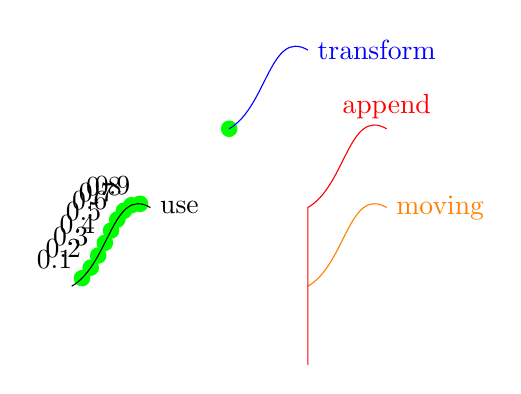
\begin{tikzpicture}
\path[spath/save=rpath] (0,0) to[out=30,in=150] (1,1);
\foreach \k in {1,...,9} {
  \fill[green] (spath cs:rpath 0.\k) circle[radius=3pt];
  \node[above left] at (spath cs:rpath 0.\k) {\(0.\k\)};
}
\fill[green] (2,2) circle[radius=3pt];
\draw[blue, spath/transform={rpath}{shift={(2,2)}}, spath/use=rpath] node[right] {transform};
\draw[orange] (3,0) [spath/use={rpath, move}] node[right] {moving};
\draw[red] (3,-1) -- +(0,2) [spath/append=rpath] node[above] {append};
\draw[spath/use=rpath] node[right] {use};
\end{tikzpicture}
\end{example}

\item Reversing.

\begin{example}
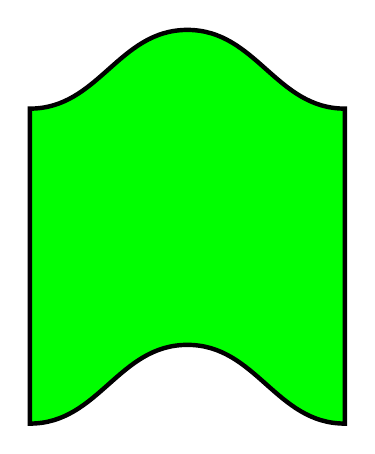
\begin{tikzpicture}
\path[spath/save=apath] (0,0) to[out=0,in=180] (2,1) to[out=0,in=180] (4,0);
\filldraw[
  green,
  draw=black,
  ultra thick,
  spath/use=apath
] -- ++(0,-4) [spath/use={apath, reverse, move, weld}] -- cycle;
\end{tikzpicture}
\end{example}

\item Transformations.

\begin{example}
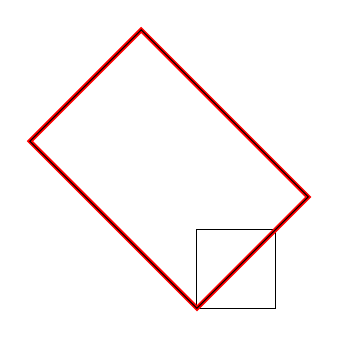
\begin{tikzpicture}
\draw[spath/save=tpath] (0,0) rectangle +(1,1);
\draw[rotate=45, xscale=2, yscale=3, ultra thick, red] (0,0) rectangle +(1,1);
\draw[
  spath/transform={tpath}{rotate=45, xscale=2, yscale=3},
  spath/use={tpath}];
\end{tikzpicture}
\end{example}

\begin{example}
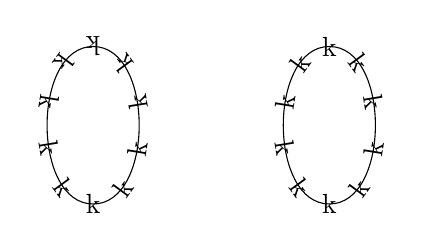
\begin{tikzpicture}
\draw[spath/save=oval] (0,0) to[out=0,in=0] (0,2) to[out=180,in=180] (0,0);
\foreach \k in {0,...,9} {
  \node[transform shape, spath/transform to={oval}{0.\k}] {k};
}
\begin{scope}[xshift = 3cm]
\draw[spath/save=soval] (0,0) to[out=0,in=0] (0,2) to[out=180,in=180] (0,0);
\foreach \k in {0,...,9} {
  \node[transform shape, spath/upright transform to={soval}{0.\k}] {k};
}
\end{scope}
\end{tikzpicture}
\end{example}

\begin{example}
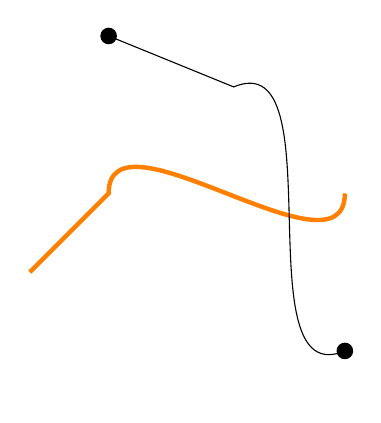
\begin{tikzpicture}
\path[draw=orange,ultra thick,spath/save=a] (3,2) -- ++(1,1) to[out=90,in=-90] ++(3,0);

\tikzset{
  spath/span={a}{(4,5)}{(7,1)}
}

\fill
(4,5) circle[radius=3pt]
(7,1) circle[radius=3pt]
;

\draw[spath/use=a];
\end{tikzpicture}
\end{example}


\item To paths.

\begin{example}
\begin{tikzpicture}
\path[draw=orange,ultra thick,spath/save=a] (3,2) -- ++(1,1) to[out=90,in=-90] ++(3,0);

\draw (0,0) -- +(1,1) to[spath/to={a}] node[pos=.6,auto] {node} ++(2,-1) -- +(3,1);
\end{tikzpicture}
\end{example}

\item Node placement.

\begin{example}
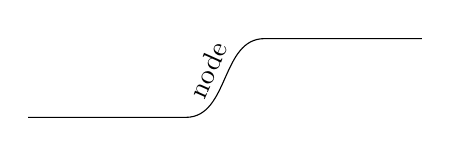
\begin{tikzpicture}
\path[spath/save=curve] (0,0) to[out=0,in=180] +(1,1);

\draw (0,0) -- (2,0) [spath/append=curve] node[pos=.5,auto,sloped] {node} -- +(2,0);

\end{tikzpicture}
\end{example}

\item Closing and adjusting paths.
\label{ex:close}

\begin{example}

\begin{tikzpicture}
\draw[line width=.2cm] (0,0) -- +(1,0) -- +(1,1) -- +(0,1) -- +(.01,.01);

\draw[line width=.2cm] (2,0) -- +(1,0) -- +(1,1) -- +(0,1) -- +(.01,.01)
-- cycle;

\draw[line width=.2cm] (4,0) -- +(1,0) -- +(1,1) -- +(0,1) -- +(.01,.01)
[spath/close=current];

\draw[line width=.2cm] (6,0) -- +(1,0) -- +(1,1) -- +(0,1) -- +(.01,.01)
[spath/adjust and close=current];
\end{tikzpicture}
\end{example}

\item Shortening.

\begin{example}
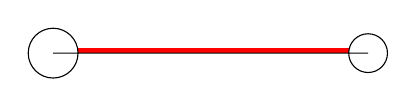
\begin{tikzpicture}
\path[spath/save=apath] (0,0) foreach \k in {1,...,4} { -- ++(1,0) +(0,0)};
\draw[
  ultra thick,
  red,
  spath/.cd,
  shorten at end={apath}{7pt},
  shorten at start={apath}{9pt},
  translate={apath}{0pt}{1pt},
  use=apath,
];
\draw (0,0) circle[radius=9pt] [spath/use=apath] circle[radius=7pt];
\end{tikzpicture}
\end{example}


\begin{example}
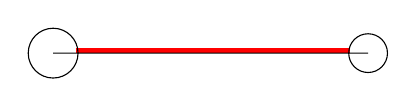
\begin{tikzpicture}
\path[spath/save=apath] (0,0) foreach \k in {1,...,4} { to[out=0,in=180] ++(1,0) +(0,0)};
\draw[
  ultra thick,
  red,
  spath/.cd,
  shorten at end={apath}{7pt},
  shorten at start={apath}{9pt},
  translate={apath}{0pt}{1pt},
  use=apath,
];
\draw (0,0) circle[radius=9pt] [spath/use=apath] circle[radius=7pt];
\end{tikzpicture}
\end{example}

\begin{example}
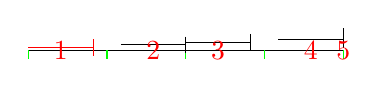
\begin{tikzpicture}
\draw[spath/save=npath] (0,0) foreach \k in {1,...,4} { -- ++(1,0) +(0,0)};
\draw[green] (0,0) -- +(0,-3pt) foreach \k in {1,...,4} { -- +(0,-3pt) ++(1,0)} -- +(0,-3pt);

\tikzset{
  spath/.cd,
  insert gaps after components={npath}{10pt}{1,3},
  get components of={npath}\components,
}

\tikzset{
  path 1/.style={
    red,
  },
}

\foreach[count=\k] \cpt in \components {
  \path[
    draw,
    path \k/.try,
    spath/.cd,
    translate=\cpt{0pt}{\k pt},
    use=\cpt,
  ] +(0,3pt) -- +(0,-3pt);
  \node[text=red] at (spath cs:{\cpt} .5) {\(\k\)};
}
\end{tikzpicture}
\end{example}

\item Intersections.

One of the main motivations for implementing the intersection routines was to provide a different way of drawing knots and links and similar diagrams.

\begin{enumerate}

\item Define the two paths for the braid (usually these will be defined with |\path|).
\begin{example}
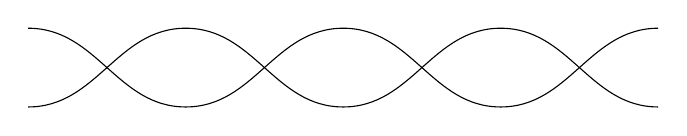
\begin{tikzpicture}[
  use Hobby shortcut,
]
\draw[spath/save global=pathA] (0,0) to[out=0,in=180] ++(2,1) to[out=0,in=180] ++(2,-1)  to[out=0,in=180] ++(2,1)  to[out=0,in=180] ++(2,-1);
\draw[spath/save global=pathB] (0,1) to[out=0,in=180] ++(2,-1) to[out=0,in=180] ++(2,1)  to[out=0,in=180] ++(2,-1)  to[out=0,in=180] ++(2,1);
\end{tikzpicture}
\end{example}

\item Split the paths at their mutual intersections and render them with a count of the components.

\begin{example}
\begin{tikzpicture}
\tikzset{
  spath/.cd,
  split at intersections={pathA}{pathB},
  get components of={pathA}\pathAcomponents,
  get components of={pathB}\pathBcomponents,
}

\foreach[count=\k] \cpt in \pathAcomponents {
  \draw[spath/use=\cpt,-Circle];
  \node[fill=white, fill opacity=.5, circle, text opacity=1] at (spath cs:{\cpt} .5) {\(\k\)};
}

\foreach[count=\k] \cpt in \pathBcomponents {
  \draw[spath/use=\cpt,-Circle];
  \node[fill=white, fill opacity=.5, circle, text opacity=1] at (spath cs:{\cpt} .5) {\(\k\)};
}
\end{tikzpicture}
\end{example}

\item Now we insert gaps after certain components in each path and then render the components.
To show that the gaps are genuine, we use a patterned background.
Although the paths were defined globally, the splitting in the previous example was local so we need to repeat it in this one.

\begin{example}
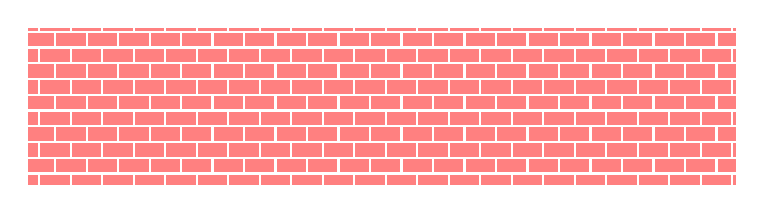
\begin{tikzpicture}
\tikzset{
  spath/.cd,
  split at intersections={pathA}{pathB},
  insert gaps after components={pathA}{5pt}{1,3},
  join components={pathA}{3,5},
  get components of={pathA}\pathAcomponents,
  insert gaps after components={pathB}{5pt}{2,4},
  join components={pathB}{2,4},
  get components of={pathB}\pathBcomponents,
}

\fill[red!50!white] (-.5,-.5) rectangle (8.5,1.5);
\fill[pattern=bricks, pattern color=white] (-.5,-.5) rectangle (8.5,1.5);

\foreach[count=\k] \cpt in \pathAcomponents {
  \draw[blue, line width=2pt,spath/use=\cpt];
  \node[fill=cyan, fill opacity=.5, circle, text opacity=1] at (spath cs:{\cpt} .3) {\(\k\)};
}

\foreach[count=\k] \cpt in \pathBcomponents {
  \draw[green, line width=2pt,spath/use=\cpt];
  \node[fill=green!50, fill opacity=.5, circle, text opacity=1] at (spath cs:{\cpt} .3) {\(\k\)};
}
\end{tikzpicture}
\end{example}
\end{enumerate}

\item This example is notable because many of the intersection points are where segments of the path end, showing that the algorithm works well even in this circumstance.

\begin{enumerate}
\item Here's the original path.
\begin{example}
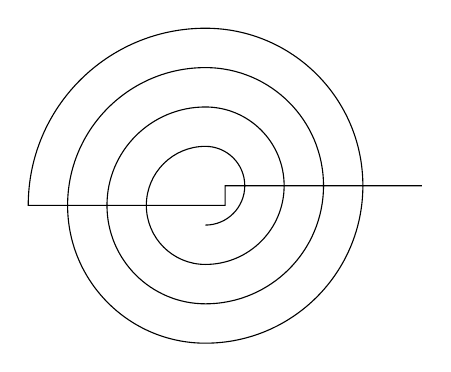
\begin{tikzpicture}
\draw[spath/save global=spiral] (5,0) -- (2.5,0) -- ++(0,-.25) -- ++(-2.5,0)
arc[radius=2.25cm,start angle=180,end angle=90]
arc[radius=2cm,start angle=90, delta angle=-180]
arc[radius=1.75cm,start angle=-90, delta angle=-180]
arc[radius=1.5cm,start angle=90, delta angle=-180]
arc[radius=1.25cm,start angle=-90, delta angle=-180]
arc[radius=1cm,start angle=90, delta angle=-180]
arc[radius=.75cm,start angle=-90, delta angle=-180]
arc[radius=.5cm,start angle=90, delta angle=-180]
;
\end{tikzpicture}
\end{example}

\item This renders labels on each component after splitting.
\begin{example}
\begin{tikzpicture}
\tikzset{
  spath/.cd,
  split at self intersections=spiral,
  get components of={spiral}\pathcomponents,
}

\foreach[count=\k] \cpt in \pathcomponents {
  \draw[spath/use=\cpt,-|];
  \node[fill=white, fill opacity=.5, circle, text opacity=1] at (spath cs:{\cpt} .5) {\(\k\)};
}
\end{tikzpicture}
\end{example}

\item Finally, we put the gaps in where we want them.

\begin{example}
\begin{tikzpicture}
\tikzset{
  spath/.cd,
  split at self intersections=spiral,
  insert gaps after components={spiral}{10pt}{1,3,5,7,10,11,14},
  spot weld=spiral,
  get components of={spiral}\pathcomponents,
}

\foreach[count=\k] \cpt in \pathcomponents {
  \draw[blue, line width=2pt,spath/use=\cpt];
}
\end{tikzpicture}
\end{example}
\end{enumerate}

\item Here's a trefoil knot, demonstrating the \texttt{knot} style that simplifies creating knots.
\begin{example}
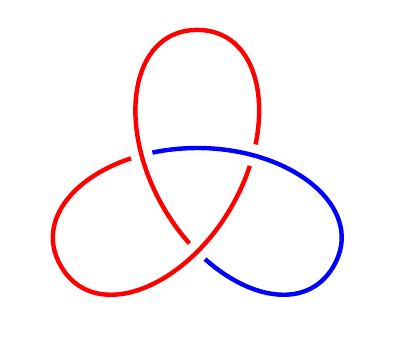
\begin{tikzpicture}[
  use Hobby shortcut,
  every trefoil component/.style={ultra thick, draw, red},
  trefoil component 1/.style={blue},
]
\path[spath/save=trefoil] ([closed]90:2) foreach \k in {1,...,3} { .. (-30+\k*240:.5) .. (90+\k*240:2) } (90:2);
\tikzset{spath/knot={trefoil}{8pt}{1,3,5}}
\end{tikzpicture}
\end{example}

\item Here's how to mark intersections of paths with ``bridges''.
\begin{example}
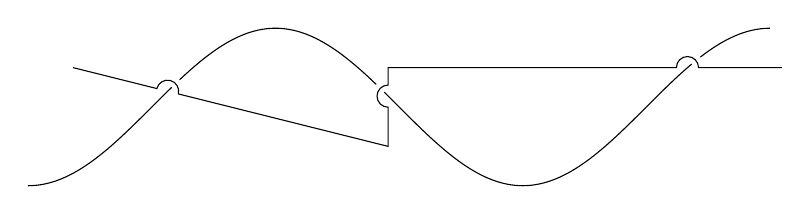
\begin{tikzpicture}
\coordinate (a) at (-1,0.5);
\coordinate (b) at (8,0.5);
\coordinate (c) at (3,-0.5);
\path[spath/save=sine]
(-1.57,-1)
cos ++(1.57,1)
sin ++(1.57,1)
cos ++(1.57,-1)
sin ++(1.57,-1)
cos ++(1.57,1)
sin ++(1.57,1);
\path[spath/save=over] (a) -- (c) |- (b);

\path[spath/save=arc] (0,0) arc[radius=1cm, start angle=180, delta angle=-180];

\tikzset{
  spath/split at intersections with={over}{sine},
  spath/insert gaps after components={over}{8pt},
  spath/join components upright with={over}{arc},
  spath/split at intersections with={sine}{over},
  spath/insert gaps after components={sine}{4pt},
}

\draw[spath/use=sine];
\draw[spath/use=over];
\end{tikzpicture}
\end{example}

\item If there are lots of paths like the previous example, here's a convenient style to put them together.
\begin{example}
\tikzset{
  bridging path/.initial=arc,
  bridging span/.initial=8pt,
  bridging gap/.initial=4pt,
  bridge/.style 2 args={
    spath/split at intersections with={#1}{#2},
    spath/insert gaps after components={#1}{\pgfkeysvalueof{/tikz/bridging span}},
    spath/join components upright with={#1}{\pgfkeysvalueof{/tikz/bridging path}},
    spath/split at intersections with={#2}{#1},
    spath/insert gaps after components={#2}{\pgfkeysvalueof{/tikz/bridging gap}},
  }
}

% If used in the preamble, this needs surrounding in \AtBeginDocument
%\AtBeginDocument{
\tikz[overlay] { \path[spath/save global=arc] (0,0) arc[radius=1cm, start angle=180, delta angle=-180]; }
%}
\begin{tikzpicture}
\path[spath/save=over] (0,0) -| ++(1,1) -| ++(-1,1) -| ++(1,1) -| ++(-1,1);
\path[spath/save=under] (.5,-.5) -- ++(0,4);
\tikzset{bridge={over}{under}}
\draw[spath/use=over];
\draw[spath/use=under];
\end{tikzpicture}
\end{example}

\end{enumerate}
  \end{document}
